% Options for packages loaded elsewhere
\PassOptionsToPackage{unicode}{hyperref}
\PassOptionsToPackage{hyphens}{url}
%
\documentclass[
]{book}
\usepackage{lmodern}
\usepackage{amssymb,amsmath}
\usepackage{ifxetex,ifluatex}
\ifnum 0\ifxetex 1\fi\ifluatex 1\fi=0 % if pdftex
  \usepackage[T1]{fontenc}
  \usepackage[utf8]{inputenc}
  \usepackage{textcomp} % provide euro and other symbols
\else % if luatex or xetex
  \usepackage{unicode-math}
  \defaultfontfeatures{Scale=MatchLowercase}
  \defaultfontfeatures[\rmfamily]{Ligatures=TeX,Scale=1}
\fi
% Use upquote if available, for straight quotes in verbatim environments
\IfFileExists{upquote.sty}{\usepackage{upquote}}{}
\IfFileExists{microtype.sty}{% use microtype if available
  \usepackage[]{microtype}
  \UseMicrotypeSet[protrusion]{basicmath} % disable protrusion for tt fonts
}{}
\makeatletter
\@ifundefined{KOMAClassName}{% if non-KOMA class
  \IfFileExists{parskip.sty}{%
    \usepackage{parskip}
  }{% else
    \setlength{\parindent}{0pt}
    \setlength{\parskip}{6pt plus 2pt minus 1pt}}
}{% if KOMA class
  \KOMAoptions{parskip=half}}
\makeatother
\usepackage{xcolor}
\IfFileExists{xurl.sty}{\usepackage{xurl}}{} % add URL line breaks if available
\IfFileExists{bookmark.sty}{\usepackage{bookmark}}{\usepackage{hyperref}}
\hypersetup{
  hidelinks,
  pdfcreator={LaTeX via pandoc}}
\urlstyle{same} % disable monospaced font for URLs
\usepackage{longtable,booktabs}
% Correct order of tables after \paragraph or \subparagraph
\usepackage{etoolbox}
\makeatletter
\patchcmd\longtable{\par}{\if@noskipsec\mbox{}\fi\par}{}{}
\makeatother
% Allow footnotes in longtable head/foot
\IfFileExists{footnotehyper.sty}{\usepackage{footnotehyper}}{\usepackage{footnote}}
\makesavenoteenv{longtable}
\usepackage{graphicx}
\makeatletter
\def\maxwidth{\ifdim\Gin@nat@width>\linewidth\linewidth\else\Gin@nat@width\fi}
\def\maxheight{\ifdim\Gin@nat@height>\textheight\textheight\else\Gin@nat@height\fi}
\makeatother
% Scale images if necessary, so that they will not overflow the page
% margins by default, and it is still possible to overwrite the defaults
% using explicit options in \includegraphics[width, height, ...]{}
\setkeys{Gin}{width=\maxwidth,height=\maxheight,keepaspectratio}
% Set default figure placement to htbp
\makeatletter
\def\fps@figure{htbp}
\makeatother
\setlength{\emergencystretch}{3em} % prevent overfull lines
\providecommand{\tightlist}{%
  \setlength{\itemsep}{0pt}\setlength{\parskip}{0pt}}
\setcounter{secnumdepth}{5}
\usepackage{booktabs}
\usepackage[]{natbib}
\bibliographystyle{apalike}

\author{}
\date{\vspace{-2.5em}}

\begin{document}

{
\setcounter{tocdepth}{1}
\tableofcontents
}
\pagebreak

\hypertarget{welcome-phage-hunters}{%
\chapter*{Welcome Phage Hunters!}\label{welcome-phage-hunters}}
\addcontentsline{toc}{chapter}{Welcome Phage Hunters!}


\includegraphics{images/redford.png}

Antimicrobial resistance is a global threat to human health and represents one of the greatest societal challenges of our time. Since their discovery at the turn of the 20th Century, bacteriophages have been used to treat bacterial infections. A contemporary renaissance of phage therapy is underway that offers a powerful tool to complement existing antibiotics and develop the next generation of targeted antimicrobials.

Phage therapy depends on the availability of a large and diverse library of isolated phages which are able to kill specific pathogenic bacterial strains. While several countries (Israel, USA, Poland, Georgia, S. Korea, France) are building or consolidating such libraries for human use, no such effort is being undertaken in the UK.

Phages for therapeutic use are typically isolated from a limited range of environments such as sewage and agricultural run-off where pathogen abundance is high, but pathogen diversity is narrow. The enormous diversity of phages in other environments remains a vast and untapped resource of potential therapeutics.

This is where you come in! During this three week project, you will isolate novel phages against a range of pathogens that cause multi-drug resistant infections. Phages will be isolated from freshwater samples that you collect around campus and the local area. You will purify the phages, extract their DNA for sequencing and then evaluate that sequencing data to determine whether or not a phage is suitable for therapeutic use.

\textbf{If a phage is discovered in your samples, you get to name it and be recorded as its Discoverer!}

This project is part of a larger Citizen Phage Library project that we recently started to rapidly develop UK capacity for providing phages for clinical use. If you wish, your phages will be recorded as part of this project. \textbf{It would be super-helpful on for the Citizen Phage Library if you would take lots of photos during the workshop!}

\hypertarget{project-aims}{%
\section*{Project Aims}\label{project-aims}}
\addcontentsline{toc}{section}{Project Aims}

\begin{enumerate}
\def\labelenumi{\arabic{enumi}.}
\tightlist
\item
  To give you all an opportunity to get into the lab and participate in research
\item
  To isolate phages that can be used for treating multi-drug resistant diseases
\item
  To be co-authors on a paper highlighting this project as a Course-based Undergraduate Research Experience
\end{enumerate}

\hypertarget{expected-learning-outcomes}{%
\section*{Expected Learning Outcomes}\label{expected-learning-outcomes}}
\addcontentsline{toc}{section}{Expected Learning Outcomes}

\begin{enumerate}
\def\labelenumi{\arabic{enumi}.}
\tightlist
\item
  Develop understanding of aseptic technique and phage isolation protocols
\item
  Develop understanding of phage therapy and its potential use in combating antimicrobial resistance
\item
  Develop bioinformatic skills to annotate and analyse phage genomic information using online tools.
\end{enumerate}

\hypertarget{your-supervisory-team-for-this-project}{%
\section*{Your Supervisory Team for this project}\label{your-supervisory-team-for-this-project}}
\addcontentsline{toc}{section}{Your Supervisory Team for this project}

\begin{itemize}
\tightlist
\item
  \textbf{Ben Temperton} - Senior Lecturer at Exeter and massive phage nerd.
\item
  \textbf{Michelle Michelsen} - PhD student in the Temperton Lab working on marine host-virus interactions and the influence of infection on cellular metabolism
\item
  \textbf{Dr Julie Fletcher} - Senior Technician in the Temperton Lab working on the Citizen Phage Library Project. Expert in infections associated with diabetic foot ulcers.
\item
  \textbf{Dr Sariqa Wagley} - Postdoctoral fellow with expertise in \emph{Vibrio} infections in aquaculture.
\item
  \textbf{Christian Fitch} - Undergraduate researcher who will be guiding you through the informatics.
\item
  \textbf{Lauren Grant} - Undergraduate researcher who will be guiding you through the informatics.
\end{itemize}

\hypertarget{house-keeping-rules}{%
\chapter*{House Keeping Rules}\label{house-keeping-rules}}
\addcontentsline{toc}{chapter}{House Keeping Rules}

\hypertarget{lab-times-and-kick-off-meeting}{%
\section*{Lab times and Kick-Off Meeting}\label{lab-times-and-kick-off-meeting}}
\addcontentsline{toc}{section}{Lab times and Kick-Off Meeting}

Lab sessions will run from \textbf{0930-1230 each day in GP108}. The kick-off meeting (Monday 17th May) where you will be handed a sampling pack will take place in \textbf{at 9:35 am in LSI Seminar Room A}. Most lab sessions are scheduled to take about 1-2 hours. Some will take the full three hour period.

\textbf{Due to the tight scheduling, there is not much opportunity to catch-up}. Each day of the workshop builds upon the previous day. The schedule is designed so that we can get DNA to the sequencing centre in time for it to be processed with sufficient time after for analysis. Social distancing also prevents us from buddying-up. So, if you miss a day, we will do what we can to catch you up, but there are no guarantees. If you are unable to see your phage isolation all the way through due to unforseen circumstances, you will still be able to participate in the genome annotation and informatics sessions.

\hypertarget{safe-working-practices}{%
\section*{Safe working practices}\label{safe-working-practices}}
\addcontentsline{toc}{section}{Safe working practices}

Each of you will be assigned a pathogen to use for phage isolation. Please make sure you read the appropriate Risk Assessment BEFORE you start handling your cultures. \protect\hyperlink{risk-assessment}{They can be found here}.

Please also ensure that you have read the appropriate sections of the Risk Assessment document entitled \texttt{General\ considerations\ for\ working\ with\ Containment\ Level\ 2\ pathogens} before performing the work.

\hypertarget{working-in-a-covid-secure-manner}{%
\section*{Working in a COVID-secure manner}\label{working-in-a-covid-secure-manner}}
\addcontentsline{toc}{section}{Working in a COVID-secure manner}

\begin{itemize}
\tightlist
\item
  COVID-19 safety policies remain in place, including \textbf{face-coverings which must be worn} inside University buildings.
\item
  Social distancing rules remain in place in the lab. Please keep to your work area and be mindful of others when moving around.
\item
  \textbf{If you feel unwell, or develop any symptoms associated with COVID19, or if you have a positive test, STAY AWAY}
\item
  It is recommended that you get regularly tested during the workshop. You can book a free test on-campus \href{https://www.exeter.ac.uk/coronavirus/times/}{here}.
\item
  Please enter GP108 by coming up the rear staircase to avoid heavy footfall in the GP lobby. We will make sure the outside door is open so you can get into the lab. You can use the lockers outside for your bags.
\item
  There are clean lab coats in the lab, which you will wear for your work that day, then put them in the laundry bin when you are finished.
\item
  There are chemgene spray bottles and blue rolls for you to clean the bench before you start work and after you have completed work before you leave.
\end{itemize}

\hypertarget{aseptic-technique}{%
\section*{Aseptic technique}\label{aseptic-technique}}
\addcontentsline{toc}{section}{Aseptic technique}

We will demonstrate the following in the sessions:

\begin{itemize}
\tightlist
\item
  Mixing by pipetting
\item
  Working under a flame.
\item
  Streaking a host onto agar
\end{itemize}

Demonstrations will occur at the start of each session at \textbf{09:40}.

\hypertarget{phage-enrichment}{%
\chapter{Phage Enrichment}\label{phage-enrichment}}

\hypertarget{monday-17th-may}{%
\section{Monday 17th May}\label{monday-17th-may}}

There will be a 1-hour presentation introducing you to the project. This will be held \textbf{at 9:35 am in LSI Seminar Room A}. You will also be provided with a sampling kit containing three jars. The aim is for each student to collect three samples of freshwater. \textbf{One} of these should be from one of the ponds on campus. Try not to all sample the same pond! The other two can be from other sources near your homes or around Exeter. They can include ponds, rivers, bird baths, puddles etc. Each sample will need to be at least 25 mL (each jar holds 40 mL).

When picking your sample site, it is worth noting that following heavy rainfall, many wastewater treatment plants have storm overflows that feed into rivers and streams. This makes these regions excellent hunting grounds for new phages. \href{https://arcg.is/1He0XL}{There is a resource for finding such areas (in the interests of water safety) here}. If we have rainfall just before sampling, it might be worth considering sites found on this map in the local region.

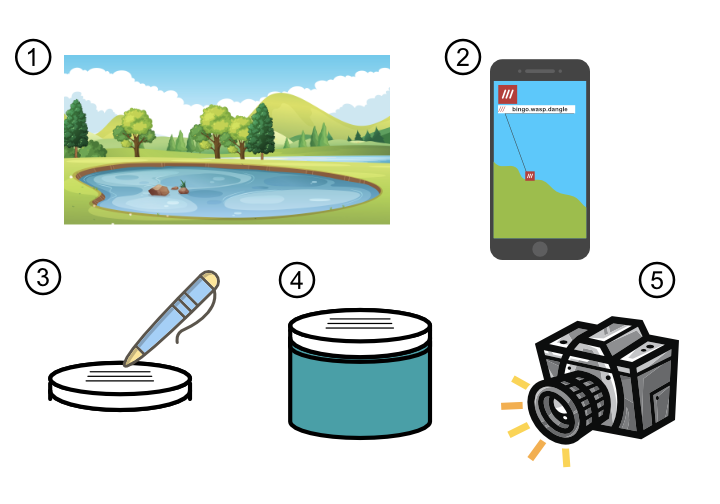
\includegraphics{images/sampling.png}

At each sample site,

\begin{itemize}
\tightlist
\item[$\square$]
  \textbf{Step 1}: Find an interesting sampling site
\item[$\square$]
  \textbf{Step 2}: Record the location using the \href{https://what3words.com/}{What3Words} app on your phone.This will be used as the name of the sample.
\item[$\square$]
  \textbf{Step 3}: Write the three words on the lid of the jar using the waterproof lab pen in your kit, as well as the sample date.
\item[$\square$]
  \textbf{Step 4}: Fill the jar with water and make sure the lid is tightly fastened.
\item[$\square$]
  \textbf{Step 5}: Take a photo of the sample site to remind you of what it was you sampled.
\end{itemize}

When you get home, keep the samples in your fridge overnight.

Record the details of your sample on the Sample tab on the \href{https://docs.google.com/spreadsheets/d/1V6doztAX4AQ5657eH5r0GbJj_GnfMxTe4eKh7metXl0/edit?usp=sharing}{Google sheet here}. Make sure you provide the What3Words address, the date and a brief description of the sample, as well as your name. You do not need to supply a sample number - these will be assigned once all samples are collected.

If you want to register your samples as part of the Citizen Phage Library project, you can also register them on the CPL portal. This is currently hosted at the university, so you'll need to be on the VPN or on University campus.

\begin{enumerate}
\def\labelenumi{\arabic{enumi}.}
\tightlist
\item
  Make sure you are either on campus or on the \href{https://www.exeter.ac.uk/it/howdoi/vpn/}{University VPN}
\item
  Go to \href{http://144.173.115.131/}{this site}
\item
  Click on `Sign In'
\item
  Click on `Sign Up'
\item
  Enter a username, email address and choose a password
\item
  A confirmation email will be sent to your email address - click on the link it contains to complete registration and it should take you to your account page.
\item
  You need to register your sampling kit before you register samples, so select the `Order or register a sampling kit' button.
\item
  Find your Sample Kit ID on the side of your sampling kit and type it in (e.g.~K-00001)
\item
  Click submit - this registers that kit ID with your account.
\item
  For each sample, click on `Register your samples'.
\item
  Enter the What3Words address, the date taken and give a description of the sample. Choose the sample picture for uploading. Your registered Sample Kit should be selected by default.
\item
  Press Submit.
\end{enumerate}

\hypertarget{tuesday-18th-may}{%
\section{Tuesday 18th May}\label{tuesday-18th-may}}

The aim of this session is to prepare your samples for phage hunting. This involves removing solid debris and bacteria by centrifugation and filtering, leaving only the phages (which are smaller than the filter size) in the filtrate. Each sample will be aliquoted into 15 aliquots (one per student).

At the end, you should have three lots of 15 1.5 mL microcentrifuge tubes. These will then be distributed between the students so each student can test each sample on their designated bacterial host.

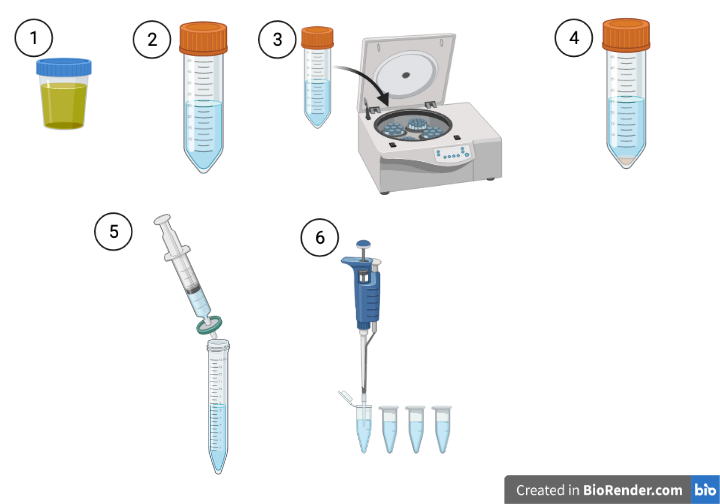
\includegraphics{images/sample-preparation.png}

\begin{itemize}
\tightlist
\item[$\square$]
  \textbf{Step 1}: Bring your samples back to the lab
\item[$\square$]
  \textbf{Step 2}: Transfer each sample to a 50 mL Falcon tube. Fill it up to the 40 mL mark. Samples need to contain the same amount of liquid to ensure balancing in the centrifuge. Label each tube with the sample number and your name. Make sure the lid is securely fastened. Draw an arrow on the lid facing outwards - this will point to where your pellet will be once it has been centrifuged, so you can avoid disturbing it.
\item[$\square$]
  \textbf{Step 3}: Place your sample in the rack at the front of the lab. These will then be centrifuged for 30 mins at 10,000 x g to pellet the solid material and bacterial cells. The phages will remain in the supernatant because they are much smaller.
\item[$\square$]
  \textbf{Step 4}: Retrieve your samples from the rack at the front and carefully carry them to your work area, being careful not to disturb the pellet.
\item[$\square$]
  \textbf{Step 5}: Using a luer-lock syringe, draw up supernatant from one of the samples. Open the syringe filter and lock the syringe into it. Push the syringe down, collecting the filtrate in a fresh tube. You need about 20 mL of filtrate. If the syringe becomes too difficult to push down, it is likely the filter is clogged. To put a new filter on, draw up the syringe slightly so it isn't dripping, then unlock the syringe filter and fit a fresh one.
\item[$\square$]
  \textbf{Step 6}: Using a 1000 µL pipettor, transfer 15 aliquots of 1000 µL of sample into 1.5 mL lo-bind microcentrifuge tube. Label the top of the tube with the sample number and your initials.
\end{itemize}

Repeat this process for the remaining samples.

When your samples have been aliquoted, take them to the front of the room in the rack. We will then organise them into sample collections for each student.

Place your Falcon tubes in the bucket provided - this allows us to clean them and autoclave them for re-use to save on plastic waste.

Return your sample jars and sampling kit boxes to the front so they can be reused.

\hypertarget{wednedsay-19th-may}{%
\section{Wednedsay 19th May}\label{wednedsay-19th-may}}

The aim of this session is to set up an overnight enrichment of each sample for a pathogen that has been assigned to you. An aliquot of sample is placed into a well in a deep-well plate and mixed with an overnight culture of pathogen and a final concentration of 1 \(\times\) LB medium + 10 mM \(MgCl_{2}\) + 30 mM \(CaCl_{2}\). Any phages in the sample capable of infecting your pathogen will infect it, undergo the lytic cycle and replicate. Over several cycles of lytic infection, the number of phages for your pathogen will be vastly enriched. In this way, we can isolate rare phages from the environment.

To see which pathogen you have been assigned, visit the `Assigned Pathogens' tab on the \href{https://docs.google.com/spreadsheets/d/1V6doztAX4AQ5657eH5r0GbJj_GnfMxTe4eKh7metXl0/edit?usp=sharing}{Google Sheet here}

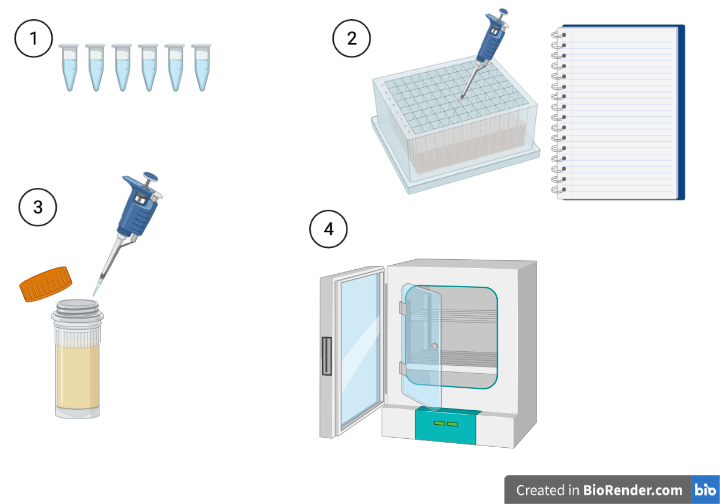
\includegraphics{images/enrichment-1.png}

\begin{itemize}
\tightlist
\item[$\square$]
  \textbf{Step 1a}: Collect your sample pack from the front. This comprises a 1.5 mL microcentrifuge tube from each sample collected by the students, plus a negative control (autoclaved MilliQ water).
\item[$\square$]
  \textbf{Step 1b}: Label your 96 well plate with your name and the name of the pathogen using labelling tape. This is so we can return your plate to you from the overnight incubation step.
\item[$\square$]
  \textbf{Step 2a}: Work out how many wells you need for your samples, plus the negative control. For each sample you have, aliquot \textbf{500 µL} of 3 \(\times\) LB + 30 mM \(MgCl_{2}\) + 30 mM \(CaCl_{2}\) into a well. Work in rows, e.g.~place one sample in A1, the next in A2, then A3 etc. You should end up with about half your plate containing liquid. You don't need to change your pipette tip between wells.
\item[$\square$]
  \textbf{Step 2b}: Change your pipette tip and aliquot \textbf{100 µL} of pathogen culture into each well that contains liquid. Again, you can use one pipette tip for the whole plate here because the content of each well is identical.
\item[$\square$]
  \textbf{Step 2c}: Using a fresh pipette tip \textbf{for each well}, Transfer \textbf{900 µL} of one sample into a well that contains medium plus pathogen. Use the pipette to \textbf{slowly} mix the well. Record the well with the sample number in your lab books. \textbf{This is critical to track back isolated phages to the samples}.
\item[$\square$]
  \textbf{Step 2d}: Cover the plate with a seal.
\item[$\square$]
  \textbf{Step 3}: Set up your overnight culture of your pathogen for use tomorrow. To do this, aliquot 10 µL of your culture into a sterilin containing 10 mL of LB medium + 10 mM \(MgCl_{2}\) + 10 mM \(CaCl_{2}\). Label the sterilin with your name and the name of your pathogen. You can use the short name of the pathogen for this.
\item[$\square$]
  \textbf{Step 4}: Carefully carry the 96-well plate and the sterilin to the front so we can place it in an incubator overnight at 30 °C. with shaking.
\end{itemize}

\hypertarget{sewage-sample-from-countess-wear}{%
\subsection{Sewage sample from Countess Wear}\label{sewage-sample-from-countess-wear}}

Sewage is a rich source of phages that infect pathogenic bacteria. To increase the likelihood of finding phages for our pathogens, we have also prepared a sample of filtered, raw sewage using the same method you used for your samples. Raw sewage can contain harmful pathogens such as Hepatitis, so to minimise risk, we have a pre-prepared deep well plate at the front of the class. Each well in that plate contains 900 µL of centrifuged, filtered sewage and 500 µL of 3 \(\times\) LB + 30 mM \(MgCl_{2}\) + 30 mM \(CaCl_{2}\).

All you need to do is aliquot \textbf{100 µL} of your original pathogen culture into the well designated in the `Assigned Sewage Plate Well' column in the spreadsheet above. \textbf{PLEASE TAKE CARE TO ALIQUOT YOUR PATHOGEN INTO THE CORRECT WELL}. If we end up with two pathogens in the same well, we won't know which one has phages enriched for it.

\hypertarget{thursday-20th-may}{%
\section{Thursday 20th May}\label{thursday-20th-may}}

Following overnight growth, the cultures in the deep-well plate should now be enriched in phages infecting your pathogen, provided they were in the original sample. Each well will also contain substances from the original sample that made it through the 0.2 µm filter. In this next step, we will start to culture the phages against their pathogen in pure culture. We filter material from the deep-well plate through a 0.45 µm filter into a fresh plate, then add that filtrate to a fresh culture (the reason we use a 0.45 µm filter instead of a 0.2 µm filter is simply due to cost - they are much cheaper!). This is a two-stage process to ensure the phage can be propagated in pure culture.

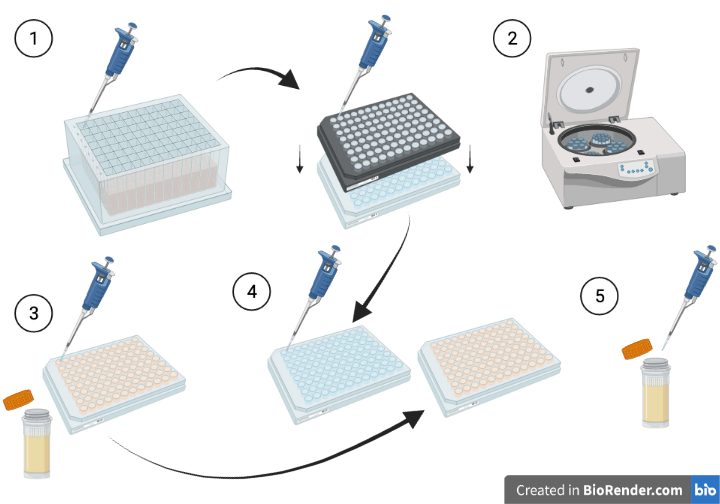
\includegraphics{images/first-filtration.png}

\begin{itemize}
\tightlist
\item[$\square$]
  \textbf{Step 1a}: Collect your deep-well plate from the front, as well as your overnight culture and return it to your work area.
\item[$\square$]
  \textbf{Step 1b}: Open up a 0.45 µm filter plate and place it on top of a sterile 96-well plate. Write your name and pathogen directly on the bottom plate. Use label tape to tape the two plates together at the edge, just to stop them slipping apart.
\item[$\square$]
  \textbf{Step 1c}: Transfer \textbf{200 µL} from each well \textbf{into the same well position} on the filter plate. It is important that you don't pipette into a wrong well, so we can track which phages came from which samples, so work slowly and carefully. If you do make a mistake, make a note of it in your lab books so we can correct the error in the final stages.
\item[$\square$]
  \textbf{Step 1d}: Cover your filter plate with a seal and return it to the front.
\item[$\square$]
  \textbf{Step 2}: Our technicians will take your plate up to the 4th floor for centrifugation at 900 \(\times g\) for 4 minutes. This will transfer the phage lysate into the bottom plate, but keep the pathogens in the top plate. The bottom plate is then used to infect fresh cultures.
\item[$\square$]
  \textbf{Step 3a}: Label your a fresh, sterile 200 µL 96-well plate with your name and pathogen. Into each well add \textbf{190 µL} of LB + 10 mM \(MgCl_{2}\) + 10 mM \(CaCl_{2}\) per well in as many wells as you have samples. Like before work in rows so that it matches your deep-well plate.
\item[$\square$]
  \textbf{Step 3b}: Into each well add \textbf{10 µL} of overnight host culture that you prepared in Step 3 yesterday. Each well contains an identical mixture, so you can use the same pipette tip for the whole plate.
\item[$\square$]
  \textbf{Step 4a}: Using a different pipette tip for each well, transfer \textbf{5 µL} of phage lysate from each well of your bottom plate from Step 2 \textbf{into the same well position} on the plate containing LB + 10 mM \(MgCl_{2}\) + 10 mM \(CaCl_{2}\) and overnight host culture. Mix by pipetting. Again, if you make a mistake, make a note of it in your lab books so we can correct the error in the final stages.
\item[$\square$]
  \textbf{Step 4b}: Seal your plate with a plate seal.
\item[$\square$]
  \textbf{Step 5}: Set up your overnight culture of your pathogen for use tomorrow. To do this, aliquot \textbf{10 µL} of your culture into a sterilin containing 10 mL of LB medium + 10 mM \(MgCl_{2}\) + 10 mM \(CaCl_{2}\). Label the sterilin with your name and the name of your pathogen. You can use the short name of the pathogen for this.
\item[$\square$]
  \textbf{Step 6}: Return your plate and new overnight culture to the front so we can place them in an incubator.
\end{itemize}

\hypertarget{friday-21st-may}{%
\section{Friday 21st May}\label{friday-21st-may}}

In this session, we will complete the second stage of the propagation in pure culture. It is very similar to what was done the previous day, but using our 200 µL culture plate instead of a deep-well plate. We will also prepare a streak plate for continuing the work next week.

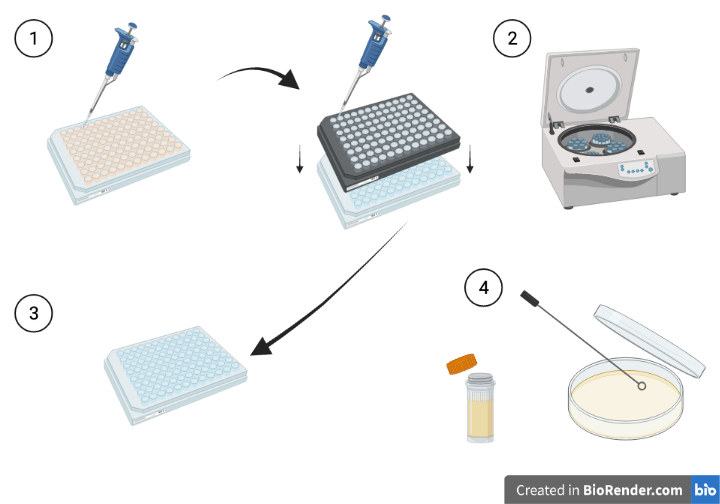
\includegraphics{images/second-filtration.png}

\begin{itemize}
\tightlist
\item[$\square$]
  \textbf{Step 1a}: Collect your plate from the front, as well as your overnight culture and return it to your work area.
\item[$\square$]
  \textbf{Step 1b}: Open up a 0.45 µm filter plate and place it on top of a sterile 96-well plate. Write your name and pathogen directly on the bottom plate. Use label tape to tape the two plates together at the edge, just to stop them slipping apart.
\item[$\square$]
  \textbf{Step 1c}: Transfer \textbf{200 µL} from each well \textbf{into the same well position} on the filter plate. It is important that you don't pipette into a wrong well, so we can track which phages came from which samples, so work slowly and carefully. If you do make a mistake, make a note of it in your lab books so we can correct the error in the final stages.
\item[$\square$]
  \textbf{Step 1d}: Cover your filter plate with a seal and return it to the front.
\item[$\square$]
  \textbf{Step 2}: Our technicians will take your plate up to the 4th floor for centrifugation at 900 \(\times g\) for 4 minutes.
\item[$\square$]
  \textbf{Step 3}: Retrieve your plate from the front and separate it from the filter plate. Cover the bottom plate with a seal. This will be used next week in the plaque assays.
\item[$\square$]
  \textbf{Step 4}: Label a petri dish containing bottom agar with your name, the date and the pathogen. Write around the edge of the `bottom' of the petri dish (remember petri dishes are cultured with their lids on the bottom). Using inoculating loops, streak out some of your overnight culture onto the plate. Close the plate and put a small piece of tape on each edge to keep the lid on.
\item[$\square$]
  \textbf{Step 5}: Return your streak petri dish and sealed phage lysate plates to the front. We will store the phage lysate at 4 °C over the weekend and incubate the petri dish culture.
\end{itemize}

\hypertarget{spot-assays-and-purification}{%
\chapter{Spot Assays and Purification}\label{spot-assays-and-purification}}

\textbf{TO BE UPDATED}

In the second week, the students will be performing spot assays and phage purification.

\hypertarget{monday-24th-may}{%
\section{Monday 24th May}\label{monday-24th-may}}

Students will set up four top agar spot plates, with 12 samples per plate (w. neg. ctrl).

\begin{itemize}
\tightlist
\item
  Students will mark plates into quadrants
\item
  Students will add 1 mL of host culture at \$OD\_\{600\} of 0.6 to 3 mL of molten top agar (0.6\% agar in LB + 10 mM \(MgCl_{2}\) + 10 mM \(CaCl_{2}\)), vortex briefly and then pour onto bottom plate
\item
  Once the plates are set, students will spot 5 µL of phage lysate from each sample at 3 per quadrant
\item
  Plates will be incubated O/N at 37 °C for plaque formation
\end{itemize}

\hypertarget{materials-required}{%
\subsection{Materials required}\label{materials-required}}

\begin{itemize}
\tightlist
\item
  10 mL pathogen culture
\item
  5 glass test tubes with lids containing 3 mL molten agar (75 total)
\item
  5 petri dishes with bottom agar (75 total)
\item
  water bath (or heat blocks if the tubes will fit in).
\end{itemize}

\hypertarget{tuesday-25th-may}{%
\section{Tuesday 25th May}\label{tuesday-25th-may}}

Students will pick plaques and perform first round of O/N purification steps. We are going to assume a maximum of 3 phages per student.

\begin{itemize}
\tightlist
\item
  Students will take a photo of their plates to record plaque morphology
\item
  For each plaque, students will core the plaque using a pipette tip and place it in 200 µL of SM buffer in a microcentrifuge tube, before vortexing briefly.
\item
  Students will then set up a dilution series from \(10^{0}\) to \(10^{-11}\) in SM Buffer in a 96 well plate (one row per phage)
\item
  Using the same method as the spot assay, students will spot the 12 dilutions onto a single plate (so one plate per phage).
\item
  Plates will be left O/N for plaques to develop
\end{itemize}

\hypertarget{materials-required-1}{%
\subsection{Materials required}\label{materials-required-1}}

\begin{itemize}
\tightlist
\item
  10 mL pathogen culture
\item
  3 glass test tubes with lids containing 3 mL molten agar (45 total)
\item
  3 petri dishes with bottom agar (45 total)
\item
  water bath (or heat blocks if the tubes will fit in).
\item
  1 sterile 96 well plate (15 total)
\item
  3 lo-bind microcentrifuge tubes (45 total)
\end{itemize}

\hypertarget{wednesday-26th-may}{%
\section{Wednesday 26th May}\label{wednesday-26th-may}}

From each plate, students will pick plaque from the biggest dilution (fewest phages) and perform second round of O/N purification. We are going to assume a maximum of 3 phages per student.

\begin{itemize}
\tightlist
\item
  Students will take a photo of their plates to record plaque morphology
\item
  For each plaque, students will core the plaque using a pipette tip and place it in 200 µL of SM buffer in a microcentrifuge tube, before vortexing briefly.
\item
  Students will then set up a dilution series from \(10^{0}\) to \(10^{-11}\) in SM Buffer in a 96 well plate (one row per phage)
\item
  Using the same method as the spot assay, students will spot the 12 dilutions onto a single plate (so one plate per phage).
\item
  Plates will be left O/N for plaques to develop
\end{itemize}

\hypertarget{materials-required-2}{%
\subsection{Materials required}\label{materials-required-2}}

\begin{itemize}
\tightlist
\item
  10 mL pathogen culture
\item
  3 glass test tubes with lids containing 3 mL molten agar (45 total)
\item
  3 petri dishes with bottom agar (45 total)
\item
  water bath (or heat blocks if the tubes will fit in).
\item
  1 sterile 96 well plate (15 total)
\item
  3 lo-bind microcentrifuge tubes (45 total)
\end{itemize}

\hypertarget{thursday-27th-may}{%
\section{Thursday 27th May}\label{thursday-27th-may}}

From each plate, students will pick plaque from the biggest dilution (fewest phages) and perform third round of O/N purification. We are going to assume a maximum of 3 phages per student.

\begin{itemize}
\tightlist
\item
  Students will take a photo of their plates to record plaque morphology
\item
  For each plaque, students will core the plaque using a pipette tip and place it in 200 µL of SM buffer in a microcentrifuge tube, before vortexing briefly.
\item
  Students will then set up a dilution series from \(10^{0}\) to \(10^{-11}\) in SM Buffer in a 96 well plate (one row per phage)
\item
  Using the same method as the spot assay, students will spot the 12 dilutions onto a single plate (so one plate per phage).
\item
  Plates will be left O/N for plaques to develop
\item
  Students will set up O/N cultures of host
\end{itemize}

\hypertarget{materials-required-3}{%
\subsection{Materials required}\label{materials-required-3}}

\begin{itemize}
\tightlist
\item
  10 mL pathogen culture
\item
  3 glass test tubes with lids containing 3 mL molten agar (45 total)
\item
  3 petri dishes with bottom agar (45 total)
\item
  water bath (or heat blocks if the tubes will fit in).
\item
  1 sterile 96 well plate (15 total)
\item
  3 lo-bind microcentrifuge tubes (45 total)
\item
  2 sterilins containing 10 mL LB + 10 mM \(MgCl_{2}\) + 10 mM \(CaCl_{2}\) (30 total)
\end{itemize}

\hypertarget{friday-28th-may}{%
\section{Friday 28th May}\label{friday-28th-may}}

From each plate, students will pick plaque from the biggest dilution (fewest phages) and bulk it up on hosts overnight.

\begin{itemize}
\tightlist
\item
  Students will take a photo of their plates to record plaque morphology. These will also be used to determine approximate PFU counts.
\item
  Students will pick plaque from the biggest dilution (fewest phages) and add it to 50 mL of LB + 10 mM \(MgCl_{2}\) + 10 mM \(CaCl_{2}\), amended with 1 mL of O/N host culture.
\item
  Cultures will be grown O/N at 30 °C
\end{itemize}

The next day (Saturday), BT and team will go in and centrifuge the samples down and prepare for each phage 1 x 50 mL tubes of lysate, filtered through a 0.2 µm syringe filter. We will prepare 3 x 2 mL phage stocks in acid washed, autoclaved amber glass vials.

\textbf{200 µL of each phage filtrate will be provided to the imaging centre.}

\hypertarget{materials-required-4}{%
\subsection{Materials required}\label{materials-required-4}}

\begin{itemize}
\tightlist
\item
  3 x 50 mL LB + 10 mM \(MgCl_{2}\) + 10 mM \(CaCl_{2}\) (2L total)
\item
  3 x 50 mL falcon tubes (45 total)
\item
  3 x 0.2 µm syringe filter (45 total)
\item
  3 x 25 mL syringe with luer lock (45 total).
\item
  3 x 2 mL amber glass vials
\end{itemize}

\hypertarget{phage-purification-and-dna-extraction}{%
\chapter{Phage Purification and DNA extraction}\label{phage-purification-and-dna-extraction}}

\textbf{TO BE UPDATED}

In the third week, the students will perform DNA extractions on phages

\hypertarget{tuesday-1st-june}{%
\section{Tuesday 1st June}\label{tuesday-1st-june}}

Students will test their lysate for estimating PFU and begin phage DNA precipitation

\begin{itemize}
\tightlist
\item
  Students will prepare a dilution series of their phages as before and spot them in triplicate across 3 plates
\item
  Students will transfer 30 mL of lysate to a fresh Falcon tube
\item
  Students will add 15 µL of nuclease solution and incubate at 37 °C for 30 mins
\item
  Students will then add 15 mL of precipitant solution to each tube and mix gently by inversion
\item
  Samples will be incubated at 4 °C O/N
\end{itemize}

\hypertarget{materials-required-5}{%
\subsection{Materials required}\label{materials-required-5}}

\begin{itemize}
\tightlist
\item
  10 mL pathogen culture
\item
  3 glass test tubes with lids containing 3 mL molten agar (45 total)
\item
  3 petri dishes with bottom agar (45 total)
\item
  water bath (or heat blocks if the tubes will fit in).
\item
  1 sterile 96 well plate (15 total)
\item
  3 x Falcon tube (45 total)
\item
  50 µL of nuclease solution (750 µL total)
\item
  50 mL of precipitant solution (750 mL total)
\end{itemize}

\hypertarget{wednesday-2nd-june}{%
\section{Wednesday 2nd June}\label{wednesday-2nd-june}}

Students will extract DNA using the Promega Wizard kit using \href{https://cpt.tamu.edu/wordpress/wp-content/uploads/2011/12/Phage-DNA-extraction-modified-Wizard-method-07-12-2011.pdf}{this protocol}

Depending on how many phages we isolate, we are anticipating sending two per student for sequencing, with the remaining extractions kept back for future analyses.
\#\#\# Materials required
* 3 x 500 µL resuspension buffer (5 mM \(MgSO_{4}\)) (25 mL total)
* 2 x Promega Wizard Kits.

\hypertarget{thursday-3rd-june}{%
\section{Thursday 3rd June}\label{thursday-3rd-june}}

Students will perform killing efficiency assays of their phages.

\textbf{Group photo!}

\hypertarget{friday-4th-june}{%
\section{Friday 4th June}\label{friday-4th-june}}

Christian and Lauren will provide an overview on using the tools via Zoom.

Two videos from the CPT also exist for this purpose:

\begin{itemize}
\tightlist
\item
  \href{https://t.co/F9Gv0rCHhS}{Structural Pipeline Video}
\item
  \href{https://t.co/5veyKIswWv}{Functional Pipeline Video}
\end{itemize}

\hypertarget{genome-annotation}{%
\chapter{Genome Annotation}\label{genome-annotation}}

\textbf{TO BE UPDATED}

The students will use the Centre for Phage Technology Galaxy Phage tool to annotate their genomes

\hypertarget{monday-7th-june}{%
\section{Monday 7th June}\label{monday-7th-june}}

Sequencing data comes back from the sequencing centre. BT performs assembly and read mapping and gives data to the students

\hypertarget{tuesdsay-8th---friday-11th-june}{%
\section{Tuesdsay 8th - Friday 11th June}\label{tuesdsay-8th---friday-11th-june}}

Students will embark on analysing their genomes. This will include:

\begin{enumerate}
\def\labelenumi{\arabic{enumi}.}
\tightlist
\item
  Classification using \href{https://www.genome.jp/viptree/}{VIPTree}
\item
  Identification of novel species and genera through \href{http://rhea.icbm.uni-oldenburg.de/VIRIDIC/}{VIRIDIC}
\end{enumerate}

\hypertarget{recipes-for-reagents}{%
\chapter*{Recipes for reagents}\label{recipes-for-reagents}}
\addcontentsline{toc}{chapter}{Recipes for reagents}

\hypertarget{agar-ploates}{%
\section{Agar ploates}\label{agar-ploates}}

\hypertarget{supplemental-nutrients}{%
\subsection{Supplemental nutrients}\label{supplemental-nutrients}}

\begin{itemize}
\tightlist
\item
  \(CaCl_2.2H_{2}O\): Prepare a 1M stock solution (58.8g in 400 mL), autoclave.
\item
  \(MgCl_{2}.6H_{2}O\): Prepare a 1M stock solution (81.32g in 400 mL), autoclave.
\end{itemize}

\hypertarget{to-make-800-ml-of-bottom-agar-plates}{%
\subsection{To make 800 mL of bottom agar plates:}\label{to-make-800-ml-of-bottom-agar-plates}}

To a 1L Schott bottle add:

\begin{itemize}
\tightlist
\item
  stirrer bar
\item
  20g LB broth
\item
  8g agar
\item
  784 mL MilliQ
\end{itemize}

Autoclave and cool to 55 °C in a water bath before the following in a flowhood:

\begin{itemize}
\tightlist
\item
  8 mL \(MgCl_{2}.6H_{2}O\) stock
\item
  8 mL \(CaCl_2.2H_{2}O\) stock.
\end{itemize}

Place on a magnetic stirrer for 1 min and allow to cool to RT.

\hypertarget{to-make-800-ml-of-top-agar}{%
\subsection{To make 800 mL of top agar:}\label{to-make-800-ml-of-top-agar}}

To a 1L Schott bottle add:

\begin{itemize}
\tightlist
\item
  stirrer bar
\item
  20g LB broth
\item
  4.8g agar
\item
  784 mL MilliQ
\end{itemize}

Autoclave and cool to 55 °C in a water bath before the following in a flowhood:

\begin{itemize}
\tightlist
\item
  8 mL \(MgCl_{2}.6H_{2}O\) stock
\item
  8 mL \(CaCl_2.2H_{2}O\) stock.
\end{itemize}

Place on a magnetic stirrer for 1 min and allow to cool to RT.

\hypertarget{a-note-on-agar-density-thickness}{%
\subsection{A note on agar density thickness}\label{a-note-on-agar-density-thickness}}

Abedon and Yin argue that because of modern agar extraction methods, contemporary agar is denser than old agar, so as a result plaques are smaller. They recommend instead using 1.0\% agar in the bottom layer (10g per 1000 mL) and 0.65\% agar in the top layer (6.5g in 1000 mL) \citep{Abedon2009-zt}. It is also recommended that plates are made fresh each time you need them (from microwaved agar), and that for spot assays, the phages are adsorbed to the agar as soon as it is gelled. The longer agar sits around, the drier and thus more dense it becomes. Bottom agar needs to be \textasciitilde30 mL per 9cm petri dish. If it's too thin, then the bottom agar doesn't buffer the waste products from the top agar, nor nutrient replenishment, leading to premature termination of plaque growth.

\hypertarget{precipitant-solution}{%
\section{Precipitant solution}\label{precipitant-solution}}

This is a ready-mixed 30\% w/v PEG-8000, 3 M NaCl solution for adding to phage lysate in a 1:2 ratio precipitant:lysate (10\%PEG-8000, 1 M NaCl final conc.)

\begin{enumerate}
\def\labelenumi{\arabic{enumi}.}
\tightlist
\item
  In a sterilized 500 mL bottle add 330 mL of autoclaved MilliQ and 105 g of NaCl and dissolve.
\item
  Add 180g of PEG8000, cap bottle and shake.
\item
  Incubate bottle in a 60 °C waterbath for 3 hours, shaking occasionally
\item
  Remove and let cool to RT, shaking occasionally
\item
  Add autoclaved MilliQ to 600 mL and store at RT.
\end{enumerate}

\hypertarget{beef-resuspension-solution}{%
\section{Beef resuspension solution}\label{beef-resuspension-solution}}

This is based on the recipe from \citep{Williamson2003-fu}. For each sample of 25g:

\begin{enumerate}
\def\labelenumi{\arabic{enumi}.}
\tightlist
\item
  To a 500 mL Duran add the following:
\end{enumerate}

\begin{itemize}
\tightlist
\item
  25g of beef extract
\item
  3.35g of \(Na_{2}HPO_{4}\cdot7H_{2}O\)
\item
  0.3g of citric acid
\end{itemize}

\begin{enumerate}
\def\labelenumi{\arabic{enumi}.}
\setcounter{enumi}{1}
\tightlist
\item
  Add 250 mL of autoclaved MQ
\item
  Add a stirrer bar
\item
  Mix until completely dissolved and adjust pH to 7.2
\end{enumerate}

\hypertarget{protocols}{%
\chapter*{Protocols}\label{protocols}}
\addcontentsline{toc}{chapter}{Protocols}

\hypertarget{preparing-phages-from-environmental-samples}{%
\section{Preparing phages from environmental samples}\label{preparing-phages-from-environmental-samples}}

\textbf{Note: Due to the need to centrifuge samples in a fixed rotor, you can only process \emph{eight} samples at any one time}

Please read all associated Risk Assessments related to the pathogens of interest before proceeding.

\hypertarget{solid-samples}{%
\subsection{Solid Samples}\label{solid-samples}}

This method is adapted from \citep{Guzman2007-na}. The proteins in the beef extract help phages desorb from solid material. Proteinaceous substances within the beef extract and those that desorb with the phages can interfere with downstream molecular analyses on large samples (e.g.~PCR) \citep{Goller2020-wx}, but for phage isolation, this isn't a problem (and beef extract is more cost effective than using PBS + BSA).

\begin{enumerate}
\def\labelenumi{\arabic{enumi}.}
\tightlist
\item
  Aliquot 10-25g of sample into a 250 mL Duran, with a magnetic stirrer
\item
  Add 1:10 w/v \protect\hyperlink{beef-resuspension-solution}{10\% beef resuspension solution (pH 7.2)}
\item
  Homogenise the sample by magnetic stirring for 20 mins at RT with sufficient speed to develop a vortex (500-900 rpm)
\item
  Transfer to 50 mL falcon tubes or larger vessels and centrifuge at 4080 xg for 10 mins at 4 °C. This stage is just to get rid of the bulk material, so can be done in the benchtop centrifuge in GP211.
\item
  Pass the supernatant through a Pluriselect 40 µm mesh filter into a fresh 50 mL Falcon tube to the 40 mL mark. Draw an arrow on the lid and mark the side where the pellet is going to be.
\item
  Centrifuge at 10,000 xg for 30 mins at 4 °C. This requires the ThermoScientific Multifuge X3R on the 4th floor.
\item
  In a flow hood, filter through a 0.2 µm PES filter into an acid-washed and autoclaved 20 mL amber glass vial (Fisher 11503552). You may have to re-centrifuge if it's really clogging the filter. Use a luer-lock syringe and filter for this to avoid it popping off and spraying everywhere! You may need to use a second filter if it starts to clog.
\item
  Label the glass vial with the \href{https://what3words.com/}{What3Words} label. Also on the side, write the date it was processed and your name.
\item
  Store at 4 °C in the dark in the CPL sample box
  \newpage
\end{enumerate}

\hypertarget{liquid-samples}{%
\subsection{Liquid Samples}\label{liquid-samples}}

\begin{enumerate}
\def\labelenumi{\arabic{enumi}.}
\tightlist
\item
  Aliquot sample into a 50 mL Falcon tube. Draw an arrow on the lid and mark the side where the pellet is going to be.
\item
  Top up to 45 mL with pH 7.5 buffer if necessary
\item
  Centrifuge at 10,000 xg for 30 mins at 4 °C. This requires the ThermoScientific Multifuge X3R on the 4th floor.
\item
  Pour supernatant into 20 mL syringe fitted with 0.2 µm PES filter
\item
  In a flow hood, filter through a 0.2 µm PES filter into an acid-washed and autoclaved 20 mL amber glass vial (Fisher 11503552). You may have to re-centrifuge if it's really clogging the filter. Use a luer-lock syringe and filter for this to avoid it popping off and spraying everywhere!
\item
  Label the glass vial with the \href{https://what3words.com/}{What3Words} label. Also on the side, write the date it was processed and your name.
\item
  Store at 4 °C in the dark in the CPL sample box
  \newpage
\end{enumerate}

\hypertarget{initial-phage-enrichment-using-2.2-ml-deep-well-plates-or-7-ml-sterilins}{%
\section{1. Initial phage enrichment (using 2.2 mL deep well plates or 7 mL sterilins)}\label{initial-phage-enrichment-using-2.2-ml-deep-well-plates-or-7-ml-sterilins}}

This method is based off this work \citep{Olsen2020-dh} and allows for the screening of one or more host strains against up to 94 samples (plus a blank and a positive control). Briefly, into each well we are adding LB medium into filtered sample that contains phages, then adding in an overnight culture of the pathogen of interest. If there are phages in the sample that infect the host, they will replicate and thus increase in abundance within the well. Subsequent steps then purify these enriched phages.

For a negative control, you want to use a sample that has no phages in it. DI water is recommended for this. You also want to run a positive control (to show that phages can be amplified and plated). For this, you can use a phage lysate that has been previously isolated on the host of interest. Spike 10 µL of previous phage lysate into 1340 µL of DI water as your positive control.

If you do not have a phage isolated on the pathogen of interest, it is recommended that you use a positive control consisting of 10 µL of T4 lysate into 1340 µL of DI. You will then need a well on your plate that contains an enrichment of \emph{E. coli} BW25113. You'll also need to include this in subsequent plaque assay steps.

\begin{enumerate}
\def\labelenumi{\arabic{enumi}.}
\tightlist
\item
  Make an O/N culture of your host of interest in LB medium at 37 °C on an orbital shaker. The required volume per host is 110 µL \(\times\) the number of samples being tested, plus one negative control and one positive. So for 10 samples plus controls, you will need \textasciitilde2 mL of host culture.
\item
  Make a 40 mL solution of 0.25 M \(CaCl_2\) and 0.25 M \(MgCl_2\) as follows:
\end{enumerate}

\begin{itemize}
\tightlist
\item
  10 mL 1M \(CaCl_2\)
\item
  10 mL 1M \(MgCl_2\)
\item
  20 mL DI water
\item
  Vortex and filter sterilize through a 0.22 µm syringe filter.
\end{itemize}

\begin{enumerate}
\def\labelenumi{\arabic{enumi}.}
\setcounter{enumi}{2}
\tightlist
\item
  The next day, unwrap an autoclaved 2.2 ml deep well 96-well plate (make sure you have the right ones! The wells are square. The ones with round wells don't hold enough liquid) in a flow hood.
\item
  Place 1350 µL of a 0.45 µm filtered sample into each well. For every strain of host, you need a negative control well (1350 µL of DI water). It's worth thinking about the final spot plaque assays when laying out the plate. It's easier to have a whole row or a whole column with a single host strain, as that way, you can spot an entire row/column onto the same plate, rather than having to cherry-pick samples.
\item
  To each well, add 80 µL of a mixture of 0.25 M \(CaCl_2\) and 0.25 M \(MgCl_2\)
\item
  To each well, add in 100 µL of an O/N culture of host
\item
  To each well, add in 450 µL of 4.4x concentration LB (44g of LB in 400 mL)
\item
  Pipette up and down to mix
\item
  Cover with a plate film.
\item
  Incubate overnight at 30 °C on an orbital shaker at 200 rpm.
\item
  Set up another O/N culture of the hosts for the next day.
\end{enumerate}

\hypertarget{risk-assessment}{%
\chapter{Risk Assessments}\label{risk-assessment}}

\begin{itemize}
\tightlist
\item
  \href{RA/CL2-RA.pdf}{General considerations for working with Containment Level 2 pathogens}
\item
  \href{RA/Acinetobacter-RA.pdf}{Acinetobacter baumannii Risk Assessment}
\item
  \href{RA/Staphylococcus-RA.pdf}{Staphylococcus aureus Risk Assessment}
\item
  \href{RA/Klebisella-RA.pdf}{Klebsiella pneumoniae Risk Assesment}
\item
  \href{RA/Pseudomonas-RA.pdf}{Pseudomonas aeruginosa Risk Assesment}
\item
  \href{RA/EC-RA.pdf}{Escherichia coli Risk Assesment}
\item
  \href{RA/EF-RA.pdf}{Enterococcus faecalis Risk Assesment}
\end{itemize}

\hypertarget{host-strains}{%
\chapter*{Host strains}\label{host-strains}}
\addcontentsline{toc}{chapter}{Host strains}

Host strains will be assigned here

  \bibliography{book.bib,packages.bib}

\end{document}
